The software has been divided into two parts, the firmware for the ARM MCU with associated sensors, and an Android application which can display sensor data. These two parts utilize a Bluetooth connection to communicate their current states. For example, when the IMU calculates a new orientation, this data should be processed by the firmware, and the resulting calculations sent to the Android application over Bluetooth to be displayed to the user.

\subsection{ARM firmware}

\begin{figure}[H]
\centering
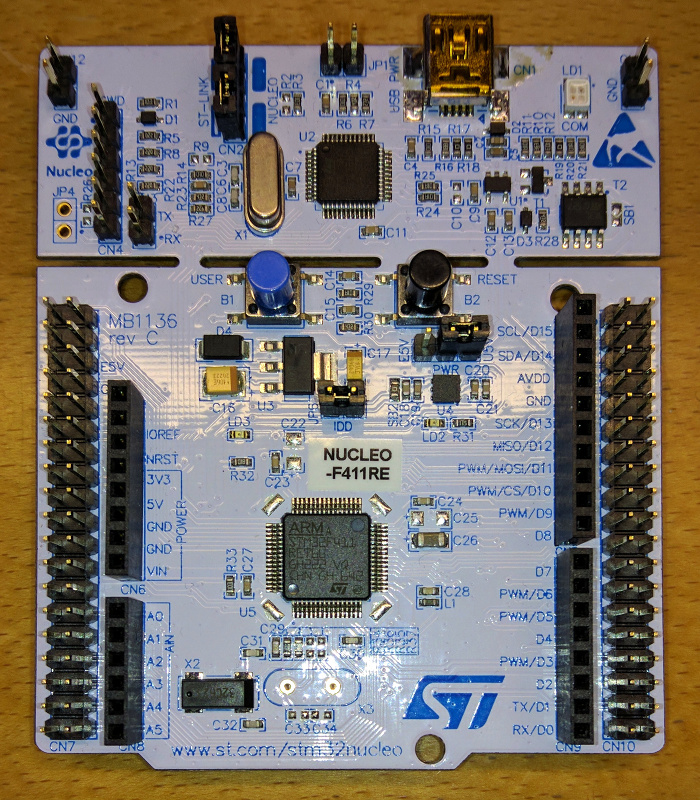
\includegraphics[width=0.6\textwidth]{Figures/stm32nucleo.jpg}
\caption{NUCLEO-F411RE development board for the ARM Cortex-M microcontroller STM32F411RE.}
\label{nucleo-board}
\end{figure}

For rapid prototyping and firmware development purposes, the NUCLEO-F411RE development board seen in figure \ref{nucleo-board} was used. This board contains break-out pins for the ARM Cortex-M microcontroller STM32F411RE, a UART to USB bridging circuit and general purpose LEDs and buttons. It is compatible with various Arudino shields as well as expansion boards developed by ST.

In order to speed up firmware development, the STM32CubeMX \cite{stm32cubemx} initialization code generator was used to set up a basic working system. This application, developed by ST, can generate C language code for setting up MCU clocks, peripherals, interrupts and similar. It is controlled by a graphical interface for setting MCU options and controlling the previously mentioned code generation.

The main challenge in working with this type of code generation is integrating it with external software libraries directly not built for it. If the library interferes with generated code by overriding settings and register values, the software may enter an undefined state and stop working. Care therefor had to be taken to only use the parts of the libraries which did not interfere. Frequent testing of any newly added functionality had to be done in order to find interfering parts.

Two libraries produced by ST were used, one for the Bluetooth module, and one for the IMU.

\subsubsection{Bluetooth}
\label{bluetooth}

\begin{figure}[H]
\centering
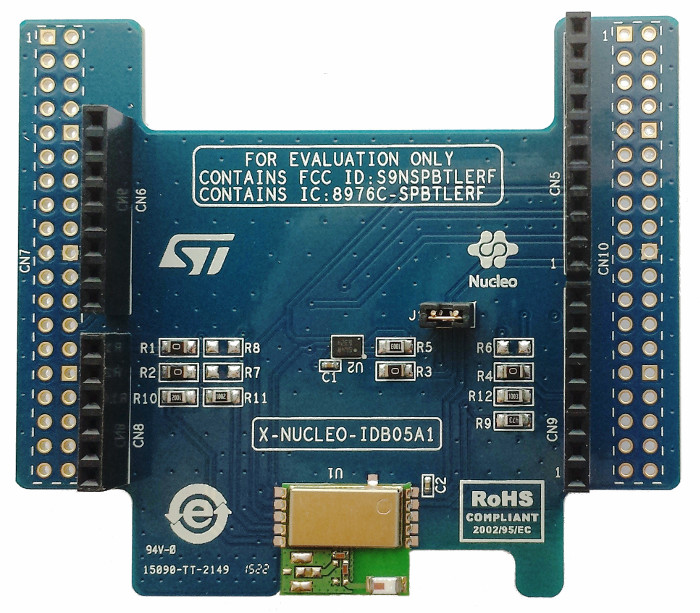
\includegraphics[width=0.6\textwidth]{Figures/x-nucleo-idb05a1.jpg}
\caption{X-NUCLEO-IDB05A1 Bluetooth Low Energy evaluation board for the STM32 Nucleo}
\label{bt-eval-board}
\end{figure}

For prototyping, the Bluetooth evaluation board X-NUCLEO-IDB05A1 \cite{x-nucleo-idb05a1} seen in figure \ref{bt-eval-board} was used, which could be stacked on top of the Nucleo board. The pins on the evaluation board connected it to an SPI port on the MCU.

To avoid having to implement the Bluetooth stack from scratch, the firmware package called X-CUBE-BLE1 \cite{x-cube-ble1} developed by ST was used. It consisted of several parts -- MCU and Bluetooth evaluation board device definitions such as named pins and ports, functions for manipulating them, a Bluetooth GATT server implementation, as well as several demo applications showing usage examples. Additionally an Android demo application for displaying sensor data from Bluetooth was available from the Google Play platform, called BlueNRG \cite{bluenrg-app}. The library code was integrated into the code generated by STM32CubeMX, added as an external library and statically linked.

While ST included example code for communicating with the Bluetooth module over SPI through interrupt based DMA transfer, this code was quite difficult to get working. Instead it was decided that blocking SPI communication were to be used, since this was much simpler to get working. The reasoning was that since the module supported a baud rate of up to 10 Mbit/s, this would be fast enough to cause miminal interference with other parts of the firmware code.

\begin{figure}[H]
\centering
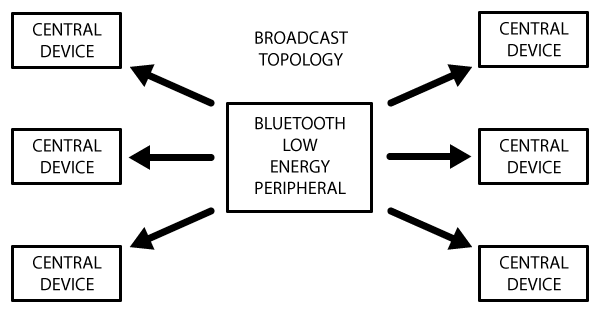
\includegraphics[width=0.6\textwidth]{Figures/bt_gap.png}
\caption{Bluetooth GAP topology.}
\label{bt-gap}
\end{figure}

\begin{figure}[H]
\centering
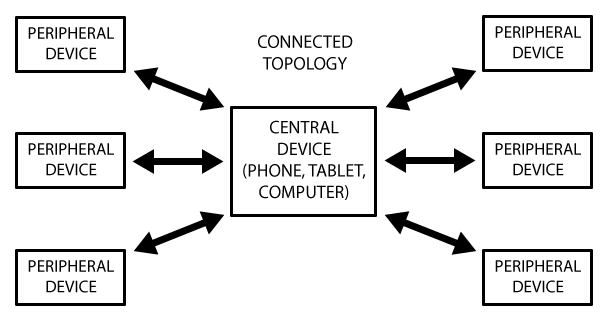
\includegraphics[width=0.6\textwidth]{Figures/bt_gatt.png}
\caption{Bluetooth GATT topology.}
\label{bt-gatt}
\end{figure}

As mentioned previously, the library implemented the Bluetooth GATT protocol. This protocol supports bidirectional communication from a single central device, in this case an Android cell phone, to several peripheral devices, such as the embedded system in this project. The library also supported the Bluetooth GAP protocol, which is a unidirectional communication protocol allowing one peripheral device to broadcast to multiple central devices. Figures \ref{bt-gatt} and \ref{bt-gap} illustrates the topological differences between these protocols.

For this project, the GATT protocol was chosen. The reasoning was that enabling the Android app to send commands to the embedded system could be useful for controlling functionality. This meant that only a single phone could be connected to the system at any time, as opposed to the GAP protocol, which would allow multiple phones to listen to the Bluetooth broadcasts. Since the embedded system is designed to be used on a small dinghy with space for a maximum of two people, this seemed like a reasonable trade-off. If the system was to be used on a larger sail boat, the GAP protocol might be more useful, since it would allow multiple passengers to listen to broadcasted sensor data.

\begin{figure}[H]
\centering
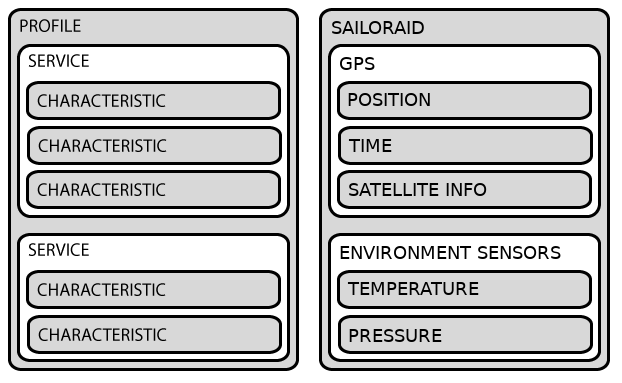
\includegraphics[width=0.6\textwidth]{Figures/bt_gatt_profile.png}
\caption{Bluetooth GATT transaction profile with usage example.}
\label{bt-gatt-profile}
\end{figure}

The GATT protocol performs transactions by nested structures called Profiles, Services and Characteristics. An example of this structure can be seen in figure \ref{bt-gatt-profile}. These structures were already implemented in the X-CUBE-BLE1 and updated by simple function calls. When new sensor data was received from e.g. the GPS or IMU devices, these functions were called at regular intervals which pushed the data to the Android app. Each profile were given a unique identifier which allowed the app to recognize which type of data was received.

\subsubsection{IMU}

\begin{figure}[H]
\centering
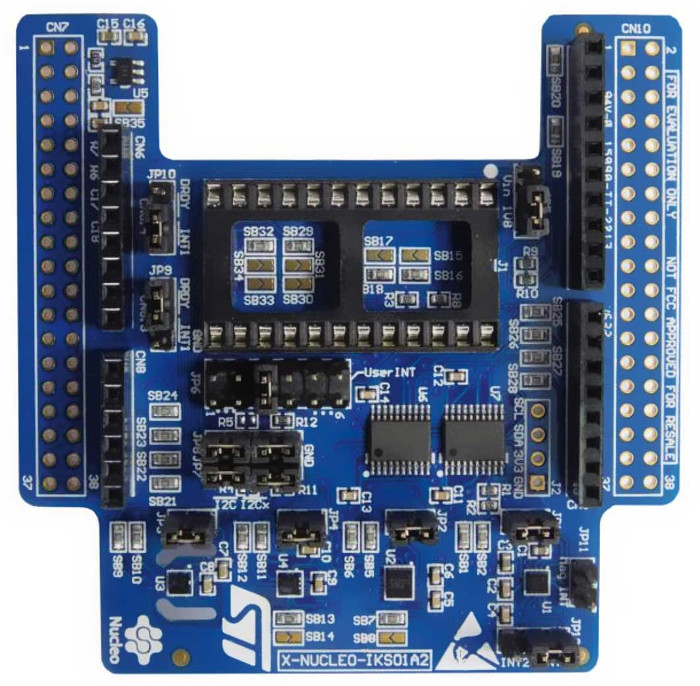
\includegraphics[width=0.6\textwidth]{Figures/x-nucleo-iks01a2.jpg}
\caption{X-NUCLEO-IKS01A2 motion MEMS and environmental sensor expansion board for the STM32 Nucleo}
\label{imu-eval-board}
\end{figure}

In order to measure the various time dependent spatial features such as orientation, acceleration and velocity, an IMU device was used. More specifically, the X-NUCLEO-IKS01A2 \cite{x-nucleo-iks01a2} evaluation board (figure \ref{imu-eval-board}) developed by ST was chosen for rapid prototyping purposes. This board included the LSM6DSL 3D accelerometer/gyroscope, the LSM303AGR 3D accelerometer/magnetometer, the HTS221 humidity and temperature sensor as well as the LPS22HB pressure sensor.

To interface the firmware with the board, the X-CUBE-MEMS1 \cite{x-cube-mems1} library developed by ST was used. This library implemented the I$^2$C communication protocol used by the previously mentioned IMU devices in the form of simple function calls, which saved a lot of development time. It was quite simple to integrate with the code generation from STM32CubeMX, only a few source definitions had to be modified. Like with the Bluetooth library (section \ref{bluetooth}) blocking communication was chosen to simplify the code, even though the MCU supported interrupt based DMA transfers. The I$^2$C operated in fast mode at 400 kHz which was thought to cause minimal interference with the rest of the system in blocking transfer mode.

An important use case for the IMU was to determine the current orientation of the dinghy. To accomplish this, a type of sensor fusion algorithm called Madgwick AHRS (section \ref{madgwick}) was used.

\subsubsection{Madgwick AHRS}
\label{madgwick}
Madgwick AHRS \cite{madgwick} is a type of sensor fusion algorithm which calculates the current orientation in space from three dimensional vectors of acceleration, angular velocity and magnetic field strength. It was developed in 2010 by Sebastian O.H. Madgwick as a more performant alternative to the Kalman filter approach. It basically integrates the angular velocity from the gyroscope, while using the accelerometer and magnetometer to create a reference to the horizontal plane. Earth’s magnetic poles provides a horizontal vector which lies on the plane, while the gravitational acceleration is the plane’s normal vector. This is then used by the algorithm to compensate for drift in gyro integration. The algorithm stores orientation in quaternions (rotation vectors with four elements), but can convert it to Euler angles, which can be more easily used.

The mathematical background of this algorithm is quite complicated and outside the scope of this report, see the official report \cite{madgwick-report} for more details.


\subsubsection{USB UART}
\label{usb-uart}
Since this project involved analyzing sensor data for developing sensor fusion algorithms, for example combining GPS and accelerometer for accurate positioning (section \ref{ekf}) and measuring water wave properties, it was important to be able to log data at a reasonably high frequency. Transferring serial commands between a computer and the MCU also helped in debugging the code. To this end, a hardware UART-over-USB chip was used, the ST-LINK/V2-1 on the Nucleo board, and FTDI FT232R on the custom project board.

At a relatively low baud rate of 115200 bps, it was determined that send and receive should both be interrupt based using DMA transfers to minimize the impact on system resources. Reception of data like key presses from a computer was handled one character at a time. The characters were appended as a string until the enter key was detected. At this point the string was matched against a list of valid commands, and the appropriate task performed -- such as sending current sensor values. Sending was implemented as a simple circular buffer which could be transferred to the UART peripheral registers using DMA.

In order to log sensor values for later analysis a simple MATLAB script was developed for listening to sensor data over the UART serial port. By inputting a serial command, the embedded system starts sending live sensor data at at constant rate. The script listens to this and logs it to a table.


\subsubsection{GPS}
The GPS module used in this project, EVA2235-H by Maestro \cite{gps} could communicate with the MCU through either I$^2$C or UART. Both protocols require only two pins to operate, but UART communication was determined to be easier to implement in code. The UART baud rate of the GPS module was set to 4800 Hz by default. While this could be changed by software there was no reason to do so. The low baud rate did however mean that blocking transmissions might cause problematic interruptions in the firmware code. To prevent this, interrupt based communication through DMA was implemented, using the same type of queuing system as the USB UART (section \ref{usb-uart}).

Data from the GPS was formatted according to the NMEA message standard. It is used by nearly all GPS devices internally, but is quite hard for a human to read. For example,
\begin{lstlisting}
GPGSA,A,3,03,22,31,23,01,06,09,11,,,,,1.9,1.2,1.5*33
GPRMC,152053.000,A,6537.0389,N,02208.0160,E,0.17,264.54,240917,,,A*6A
GPGGA,152054.000,6537.0389,N,02208.0160,E,1,08,1.2,14.0,M,25.0,M,,0000*68
\end{lstlisting}
contains three so called sentences. GPGSA contains data about the number of active satellites and positional accuracy. GPRMC and GPGGA both encode longitude, latitude, current time and date, as well as other data.

Several NMEA parsing libraries are freely available on the web. The one chosen for this project was called Libnmea \cite{libnmea} and allowed the sentences to be automatically recognized, parsed and stored into easy to use C structures.


\subsubsection{Range sensor}
\todo{todo}
